% Source of images/tikz-agent-task-matrix.svg. Rebuild with `make tikz`.
\documentclass[tikz,border=4pt]{standalone}
\begin{document}
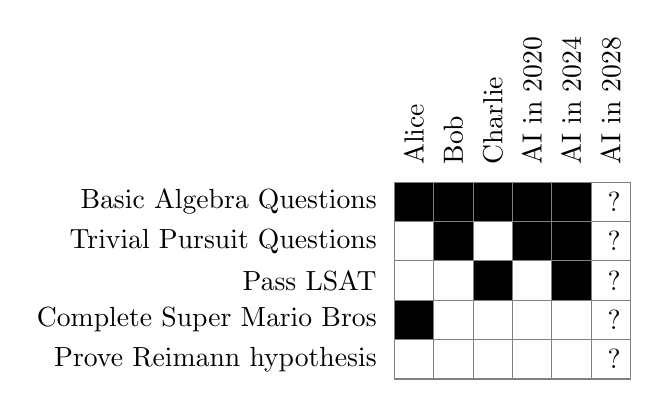
\begin{tikzpicture}[scale=0.5]
  \def\nrows{5} % Number of rows -- I tried to dynamically calculate these but it's painful
  \def\ncols{6} % Number of columns 
  \def\blackcells{1/1,1/2,1/3,1/4,1/5,2/2,2/4,2/5,3/3,4/1,3/5} % (format: column/row)
  \def\rowlabels{Basic Algebra Questions,Trivial Pursuit Questions,Pass LSAT,Complete Super Mario Bros,Prove Reimann hypothesis}
  \def\columnlabels{Alice,Bob,Charlie,AI in 2020,AI in 2024,AI in 2028}

   \foreach \i/\j in \blackcells {
      \filldraw[fill=black] (\j - 1,\nrows - \i+1) rectangle ++(1,-1); }
   \foreach \label [count=\i from 1] in \rowlabels {\node[left] at (6,\nrows - \i + 0.5) {?};}
   \foreach \label [count=\i from 1] in \rowlabels {
      \node[left] at (-0.2,\nrows - \i + 0.5) {\label};
   }
   \foreach \label [count=\j from 1] in \columnlabels {
      \node[rotate=90,right] at (\j-0.5,\nrows + 0.2) {\label}; }
   \draw[gray] (0,0) grid (\ncols,\nrows);
\end{tikzpicture}
\end{document}
